\documentclass[a4paper,12pt]{article}
\usepackage{tikz}
\usetikzlibrary{calc}
\begin{document}

\begin{figure}
\centering
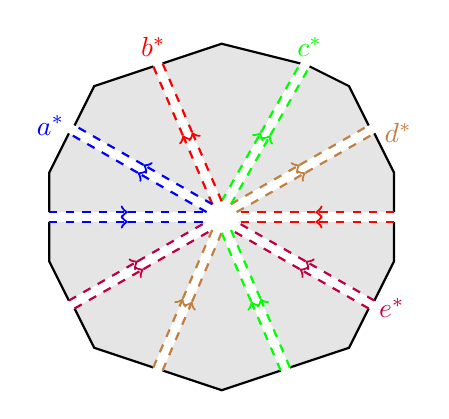
\begin{tikzpicture}[line width=0.8pt,scale=0.5]
\foreach \i in {-9,...,9}{
	\foreach \j in {-9,...,9}{
		\coordinate(v\i\j) at (\i,\j);
		\foreach \k in {0,...,9}{
			\coordinate(v\i\j\k) at ($(v\i\j)+(\k*36-18: 0.4)$);
		}
	}
}

% Numérotation : cab arête a sommet b
% Je coupe l'arête i en deux, puis décale selon sommet.


% DESSUS 
\coordinate(c11) at ($(v841)!0.5!(v761)$);
\coordinate(h11) at ($(v431)!0.5!(c11)$);
\coordinate(c12) at ($(v842)!0.5!(v762)$);
\coordinate(h12) at ($(v432)!0.5!(c12)$);

\coordinate(c22) at ($(v762)!0.5!(v572)$);
\coordinate(h22) at ($(v432)!0.5!(c22)$);
\coordinate(c23) at ($(v763)!0.5!(v573)$);
\coordinate(h23) at ($(v433)!0.5!(c23)$);

\coordinate(c33) at ($(v473)!0.5!(v163)$);
\coordinate(h33) at ($(v433)!0.5!(c33)$);
\coordinate(c34) at ($(v474)!0.5!(v164)$);
\coordinate(h34) at ($(v434)!0.5!(c34)$);

\coordinate(c44) at ($(v164)!0.5!(v044)$);
\coordinate(h44) at ($(v434)!0.5!(c44)$);
\coordinate(c45) at ($(v165)!0.5!(v045)$);
\coordinate(h45) at ($(v435)!0.5!(c45)$);


% DESSOUS

\coordinate(c11) at ($(v841)!0.5!(v761)$);
\coordinate(h11) at ($(v431)!0.5!(c11)$);
\coordinate(c12) at ($(v842)!0.5!(v762)$);
\coordinate(h12) at ($(v432)!0.5!(c12)$);

\coordinate(c22) at ($(v762)!0.5!(v572)$);
\coordinate(h22) at ($(v432)!0.5!(c22)$);
\coordinate(c23) at ($(v763)!0.5!(v573)$);
\coordinate(h23) at ($(v433)!0.5!(c23)$);

\coordinate(c33) at ($(v473)!0.5!(v163)$);
\coordinate(h33) at ($(v433)!0.5!(c33)$);
\coordinate(c34) at ($(v474)!0.5!(v164)$);
\coordinate(h34) at ($(v434)!0.5!(c34)$);

\coordinate(c66) at ($(v026)!0.5!(v106)$);
\coordinate(h66) at ($(v436)!0.5!(c66)$);
\coordinate(c67) at ($(v027)!0.5!(v107)$);
\coordinate(h67) at ($(v437)!0.5!(c67)$);

\coordinate(c77) at ($(v4-17)!0.5!(v107)$);
\coordinate(h77) at ($(v437)!0.5!(c77)$);
\coordinate(c78) at ($(v4-18)!0.5!(v108)$);
\coordinate(h78) at ($(v438)!0.5!(c78)$);

\coordinate(c88) at ($(v4-18)!0.5!(v708)$);
\coordinate(h88) at ($(v438)!0.5!(c88)$);
\coordinate(c89) at ($(v4-19)!0.5!(v709)$);
\coordinate(h89) at ($(v439)!0.5!(c89)$);

\coordinate(c99) at ($(v829)!0.5!(v709)$);
\coordinate(h99) at ($(v439)!0.5!(c99)$);
\coordinate(c90) at ($(v820)!0.5!(v700)$);
\coordinate(h90) at ($(v430)!0.5!(c90)$);


%1
\fill [gray!20](v431)--(v831)--(v841)--(c11)--cycle;
\draw (v831)--(v841)--(c11);
%b^*-1
\draw [red, dashed, ->](v831)--++(-2,0);
\draw [red, dashed](v831)++(-2,0)--(v431);
%d^*
\draw [brown, dashed, ->](v431)--(h11);
\draw [brown, dashed](h11)--(c11);

\draw [brown](c11)node[right]{$d^*$};

%2
\fill [gray!20](v432)--(c12)--(v762)--(c22)--cycle;
\draw (c12)--(v762)--(c22);
%b*^-1
\draw [brown, dashed, ->](v432)--(h12);
\draw [brown, dashed](h12)--(c12);
%c^*
\draw [green, dashed, ->](v432)--(h22);
\draw [green, dashed](h22)--(c22);

\draw [green](c22)node[above]{$c^*$};

%3
\fill [gray!20](v433)--(c23)--(v473)--(c33)--cycle;
\draw (c23)--(v473)--(c33);

%c^*
\draw [green, dashed, ->](v433)--(h23);
\draw [green, dashed](h23)--(c23);
%b*
\draw [red, dashed, ->](v433)--(h33);
\draw [red, dashed](h33)--(c33);

\draw [red](c34)node[above]{$b^*$};

%4
\fill [gray!20](v434)--(c34)--(v164)--(c44)--cycle;
\draw (c34)--(v164)--(c44);

%b*
\draw [red, dashed, ->](v434)--(h34);
\draw [red, dashed](h34)--(c34);
%a^*
\draw [blue, dashed, ->](v434)--(h44);
\draw [blue, dashed](h44)--(c44);

\draw [blue] (c44)node[left]{$a^*$};

%5
\fill [gray!20](v435)--(c45)--(v045)--(v035)--cycle;
\draw (c45)--(v045)--(v035);

%a^*
\draw [blue, dashed, ->](v435)--(h45);
\draw [blue, dashed](h45)--(c45);
%a^*-1
\draw [blue, dashed, ->](v035)--++(2,0);
\draw [blue, dashed](v035)++(2,0)--(v435);


%6
\fill [gray!20](v436)--(v036)--(v026)--(c66)--cycle;
\draw (v036)--(v026)--(c66);

%a^*-1
\draw [blue, dashed, ->](v036)--++(2,0);
\draw [blue, dashed](v036)++(2,0)--(v436);

%e*^-1
\draw [purple, dashed, ->](c66)--(h66);
\draw [purple, dashed](h66)--(v436);


%7
\fill [gray!20](v437)--(c67)--(v107)--(c77)--cycle;
\draw (c67)--(v107)--(c77);

%e*^-1
\draw [purple, dashed, ->](c67)--(h67);
\draw [purple, dashed](h67)--(v437);

%d^*-1
\draw [brown, dashed, ->](c77)--(h77);
\draw [brown, dashed](h77)--(v437);

%8
\fill [gray!20](v438)--(c78)--(v4-18)--(c88)--cycle;
\draw (c78)--(v4-18)--(c88);

%d^*-1
\draw [brown, dashed, ->](c78)--(h78);
\draw [brown, dashed](h78)--(v438);

%c^*-1
\draw [green, dashed, ->](c88)--(h88);
\draw [green, dashed](h88)--(v438);

%9
\fill [gray!20](v439)--(c89)--(v709)--(c99)--cycle;
\draw (c89)--(v709)--(c99);

%c*-1
\draw [green, dashed, ->](c89)--(h89);
\draw [green, dashed](h89)--(v439);

%e*
\draw [purple, dashed, ->](c99)--(h99);
\draw [purple, dashed](h99)--(v439);

%0
\fill [gray!20](v430)--(c90)--(v820)--(v830)--cycle;
\draw (c90)--(v820)--(v830);

%e*
\draw [purple, dashed, ->](c90)--(h90);
\draw [purple, dashed](h90)--(v430);

%b*^-1
\draw [red, dashed, ->](v830)--++(-2,0);
\draw [red, dashed](v830)++(-2,0)--(v430);

\draw [purple](c99)node[right]{$e^*$};

\end{tikzpicture}
\caption{Dualizing $abcdb^{-1}ec^{-1}d^{-1}e^{-1}a^{-1}$ into ($a$, $ba^{-1}e$, $cb^{-1}d^{-1}, dc^{-1}e^{-1}$)}
\end{figure}

\begin{figure}
\centering
\begin{tikzpicture}[line width=0.8pt,scale=0.5]
\foreach \i in {-9,...,9}{
	\foreach \j in {-9,...,9}{
		\coordinate(v\i\j) at (\i,\j);
		\foreach \k in {0,...,9}{
			\coordinate(v\i\j\k) at ($(v\i\j)+(\k*36-18: 0.4)$);
		}
	}
}

%% Cercle elliptique
\fill [gray!20] (v00) circle (1)
\draw [blue, dashed] (v00) circle (1);

\draw [blue] (v00) node[left]{$<$} node[right]{$a^*$};


%% triangle bas gauche

\fill [gray!20] (v40)--(v04)--(v44)--cycle;
\draw (v22)--(v33)--(v42)--(v33)--(v24);

%a*^-1
\draw [blue,dashed ,->](v40)--(v22)node[midway,sloped, below]{$a^{-1}$};
\draw [blue, dashed](v22)--(v04);

% b*^{-1}
\draw [red, dashed,->](v40)--(v42);
\draw [red, dashed](v42)--(v44);

%e^*
\draw [purple,dashed, ->] (v04)--(v24)node[midway, above]{$e^*$};
\draw [purple,dashed ] (v24)--(v44);

%% triangle bas droite

\fill [gray!20] (v54)--(v94)--(v50)--cycle;
\draw (v63)--(v72)--(v63)--(v52)--(v63)--(v74);

%b^*
\draw [red, dashed, ->] (v50)--(v52)node[midway, left]{$b^*$};
\draw [red, dashed] (v52)--(v54);

%c^*
\draw [green, dashed,->] (v50)--(v72)node[midway, sloped, below]{$c^*$};
\draw [green, dashed] (v72)--(v94);

%d^*
\draw [brown, dashed,->] (v94)--(v74)node[midway, above]{$d^*$};
\draw [brown, dashed] (v74)--(v54);

%% triangle haut droite
\fill [gray!20] (v55)--(v59)--(v95)--cycle;
\draw (v57)--(v75)--(v66)--(v77);

%d*^-1
\draw [brown, dashed, ->] (v95)--(v75);
\draw [brown, dashed] (v75)--(v55);

%c*^-1
\draw [green, dashed] (v55)--(v57);
\draw [green, dashed, ->] (v59)--(v57);

\draw [purple, dashed,->] (v95)--(v77);
\draw [purple, dashed] (v77)--(v59);


%\draw (v20)--(v31)--(v51)--(v53);
%\draw (2,0)--(4/3+2,4/3)--(8/3+2,4/3)--(8/3+2,8/3);
%\draw (8/3+2,4/3)--(10/3+2,2/3);

\end{tikzpicture}
\end{figure}


\begin{figure}
\centering
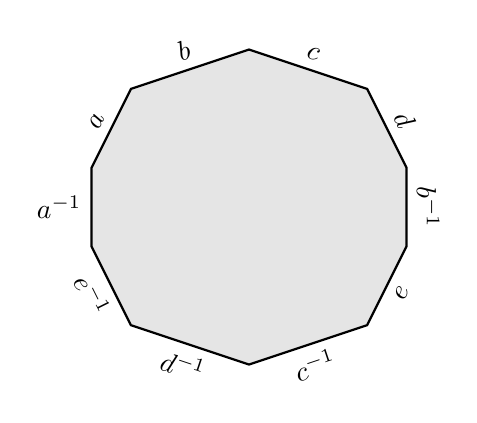
\begin{tikzpicture}[line width=0.8pt,scale=0.5]
\foreach \i in {-9,...,9}{
	\foreach \j in {-9,...,9}{
		\coordinate(v\i\j) at (\i,\j);
		\foreach \k in {0,...,9}{
			\coordinate(v\i\j\k) at ($(v\i\j)+(\k*36-18: 0.4)$);
		}
	}
}

\draw [fill=gray!20](v-80)--node[midway,sloped,below]{$e^{-1}$}(v-92)--node[midway,left]{$a^{-1}$}(v-94)--node[midway,sloped,above]{$a$}(v-86)--node[midway,sloped,above]{$b$}(v-57)--node[midway,sloped,above]{$c$}(v-26)--node[midway,sloped, above]{$d$}(v-14)--node[midway, sloped, above]{$b^{-1}$}(v-12)--node[midway,sloped, below]{$e$}(v-20)--node[midway, sloped, below]{$c^{-1}$}(v-5-1)--node[midway,sloped,below]{$d^{-1}$}cycle;

\end{tikzpicture}
\end{figure}

\end{document}

